
\chapter{Kravspecifikationer}
I dette afsnit vil gruppen vurdere, hvilke krav der skal indgå i en løsning. Heri vil der både blive opstillet krav til en optimal løsning og til en afgrænset løsning, som gruppen mener vil være realistisk, at kunne lave.

\section{Optimale løsningsforslag}
For at kunne udvilke en softwareløsning, der besvarer gruppens problemformulering, er det vigtigt at definere nogle krav til programmet. Til en optimal løsning, har gruppen vurderet, at der skal være følgende krav:
\begin{itemize}
	\item Programmet skal udvikles som en applikation til moderne smartphones, inklusiv iOS, Android og Windows Phone.
	\item Programmet skal hjælpe brugeren, til at lave en interresant rute gennem byen, vedkommende vil besøge.
	\item Programmet skal vise et overskueligt og scalerbart kort med ruten.
	\item Ruten skal udskrives i samme stil som Google Maps.
	\item Programmet skal kunne give rutevejledning undervejs på ruten. 
	\item Programmet skal kunne  downloade en offline version af den rute der er valgt, inklusiv kortet for det omkringliggende område.
\end{itemize}
Til disse krav har gruppen konstrueret nogle skitser og en beskrivelse af den optimale løsning, for at give et billede af hvordan det eventuelt kunne se ud. \newpage

Gruppen har valgt at lave den ideelle løsning på følgende måde:\newline
\newline
Brugeren bliver præsenteret for en liste over alle attraktioner i byen, sorteret efter afstand fra brugerens nuværende position, alfabetisk rækkefølge eller rating. \newline
Ratingen vil blive fundet ved at tage gennemsnittet af alle brugeres rating af den specifikke attraktion. Dette gøres for at give brugeren mulighed for at vælge de attraktioner vedkommende gerne vil se.
\newline
Programmet skal under udvælgelsen give brugeren mulighed for at læse om de enkelte attraktioner, så brugeren kan foretage informerede beslutninger om til- og fravælgelse af attraktioner.\newline
\newline
Når brugeren har valgt de attraktioner vedkommende vil besøge, udformes et kort med den korteste rute mellem disse attraktioner. På dette kort vil alle attraktioner som ligger indenfor en forudbestemt afstand til ruten, blive vist. Derefter kan brugeren tilføje nogle ekstra attraktioner, som vil blive tilføjet til den endelige rute.\newline
Dette gøres så brugeren kan udforme en mere interessant rute. Gruppen vil ikke diktere hvad den interessante rute er, men lade brugeren selv tilvælge, og derved få deres egen unikke interessante rute. \newline 


\begin{wrapfigure}{r}{0.3\textwidth}
	\vspace{-20pt}
	\begin{center}
		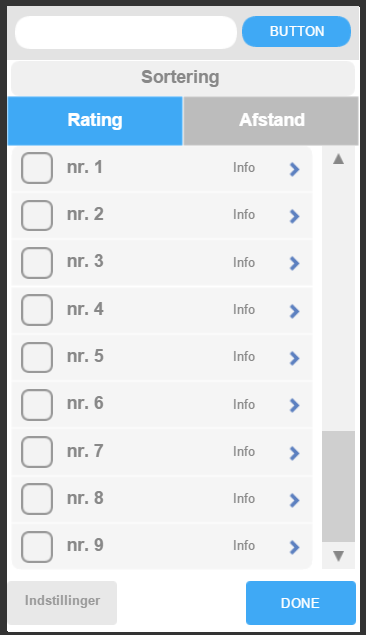
\includegraphics[scale=0.35]{start1} \newline
		\textit{Figur 3.1: Brugergrænseflade}\newline
	\end{center}
	\vspace{-20pt}
	\vspace{-20pt}
\end{wrapfigure}


Gruppen ønsker, at programmet skulle fungere på den måde, at der findes to valg muligheder, forholdsvis rating og afstand, hvoraf rating viser en række attraktioner med en værdi, baseret på hvad brugerne har valgt at rate den. Funktionen afstand, vil vise hvor stor en afstand der er fra det punkt hvor brugeren står, til en attraktion. De attraktioner, som brugeren ønsker at se, skal brugeren blot tjekke af, ved at klikke på attraktionerne, og de vil derefter blive tilføjet til den nuværende rute. Figur 3.1 viser en skitse af brugergrænsefladen. \newline
\newline
\newline
\newline

\begin{wrapfigure}{l}{0.3\textwidth}
	\vspace{-50pt}
	\begin{center}
		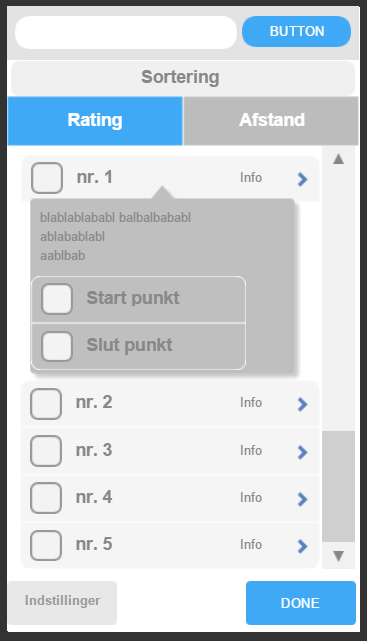
\includegraphics[scale=0.35]{start2} \newline
		\textit{Figur 3.2: \newline Udvidet brugergrænseflade}\newline
	\end{center}
	\vspace{20pt}
\end{wrapfigure}

Herudover ønsker gruppen, at der er en form for menu, som indeholder informationer omkring de forskellige attraktioner. Udover dette, skal der også være mulighed for at vælge et start- eller slutpunkt. Disse punkter skal give brugeren mulighed for at vælge, hvor brugeren ønsker at starte/slutte sin rute. Figur 3.2 viser en skitse af en udvidet brugergrænseflade.\newline
\newline
\newline
\newline
\newline

\begin{wrapfigure}{r}{0.3\textwidth}
	\vspace{-30pt}
	\begin{center}
		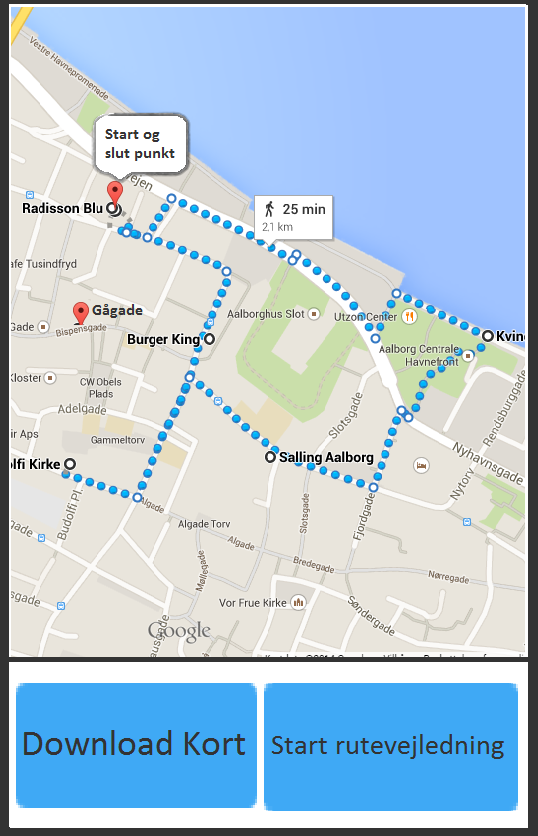
\includegraphics[scale=0.3]{rute1} \newline
		\textit{Figur 3.3: Rute - Ruten er\newline hentet fra Maps.Google.com}\newline
	\end{center}
	\vspace{0pt}
	\vspace{-100pt}
\end{wrapfigure}


Når der er valgt nogle ønskede destinationer/attraktioner, skal programmet fremvise en rute. Ruten skal vise hvor lang hele ruten er, og hvor lang tid det tager at gå ruten. Der skal desuden være to funktioner, når ruten bliver vist. Der skal være mulighed for at downloade kortet på mobilen, og derved gør det muligt at anvende programmet, uden brug af internet. Den anden funktion skal starte rutevejledningen, som fungere som en ganske almindelig GPS. En skitse af dette kan ses på figur 3.3.\newline
\newline
\newline
\newline
\newline
\newline
\newline
\newline

\begin{wrapfigure}{l}{0.3\textwidth}
	\vspace{-20pt}
	\begin{center}
		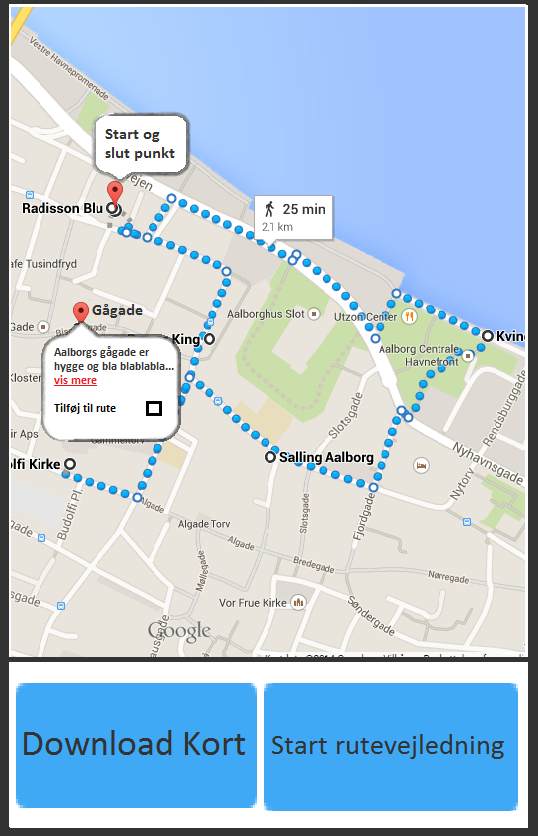
\includegraphics[scale=0.3]{rute2} \newline
		\textit{Figur 3.4: Udvidet rute - Ruten er hentet fra\newline Maps.Google.com}\newline
	\end{center}
	\vspace{-20pt}
	\vspace{-10pt}
\end{wrapfigure}

Der skal desuden også her være mulighed for at få information om attraktionerne, der er i nærheden af den valgte rute. Der skal være en "tilføj til nuværende rute"-funktion, som tilføjer de valgte attraktioner, som er i nærheden til den rute, der allerede er lavet. Figur 3.4 viser hvordan det eventuelt kunne laves. \newline
\newline
\newline
\newline
\newline
\newline
\newline
\newline
\newline
\newline
\newline
\newline


\section{Gruppens løsningsforslag}
Gruppen har gennem spørgeskema og interview fået stillet en række krav til løsningen, af respondentgruppen og VisitAalborg. 
Gennem spørgskemaet, blev det konkluderet, at det vigtigste for turister, er at de kan opleve byen på en interessant rute. 
Derudover har turistbureauet givet udtryk for, at løsningen gerne skal være så enkelt som muligt, altså færrest mulige funktioner, så brugeren ikke bliver forvirret, da de mener, at det er i turistens bedste interesse. \newline
Der er blevet stillet krav fra universitets side, om at programmet skal være et lille specifikt program i C, af høj kvalitet. Dette stemmer godt overens, med de krav der er blevet stillet fra turistbureauets side.   \newline
Ud fra dette, har gruppen opsat nogle krav for gruppens løsningsforslag, og de er som følgende:
\begin{itemize}
	\item Programmet skal kunne beregne en kort rute mellem en række punkter.
	\item Programmet skal beregne om der ligger en attraktion mindre end 100 meter fra ruten, og tilføje ekstra attraktionen til ruten, hvis brugeren ønsker det.
	\item Programmet skal som output give en liste over rutens destinationer, i den rækkefølge de skal besøges, i forhold til den korte rute.
\end{itemize}

Da dette er et P1 projekt, og gruppen er begrænset af både tid og erfaring, har gruppen valgt at begrænse softwareløsningen, på følgende punkter: 
\begin{itemize}
	\item Afstanden mellem attraktioner vil blive beregnet i fugleflugtslinje.
	\item Brugeren kan kun vælge destinationer ud fra en række forudbestemte punkter.
	\item Tekstbaseret brugergrænseflade.
\end{itemize}

På baggrund af kravene og afgrænsningen, har gruppen valgt at lave et program, som har nogle forudbestemte destinationer, der dækker over attraktioner i Aalborg, hvorefter brugeren vælger de attraktioner vedkommende ønsker at besøge. Programmet vil ud fra disse punkter, beregne en kort rute, og undersøge om der er andre attraktioner, som ligger tæt på ruten, og spørge brugeren, om det kunne være interessant at besøge disse steder. Hvis ja, vil disse punkter også blive inkluderet. På den måde får brugeren selv lov til at skabe sig den mest interessante rute. Resultatet bliver en liste over destinationerne, der står i rækkefølge, så turisten ved hvilken rækkefølge de skal besøge dem i, for at få den mest optimale rute.\newline

Det næste afsnit vil omhandle de teorier, som beskriver de formler, algoritmer og metoder, der er brugt i løsningen.
